% options:
% thesis=B bachelor's thesis
% thesis=M master's thesis
% czech thesis in Czech language
% english thesis in English language

\documentclass[thesis=B,czech]{FITthesis}[2011/06/14]

\usepackage[utf8]{inputenc} % LaTeX source encoded as UTF-8

\usepackage{graphicx} %graphics files inclusion
% \usepackage{amsmath} %advanced maths
% \usepackage{amssymb} %additional math symbols

% % list of acronyms
% \usepackage[acronym,nonumberlist,toc,numberedsection=autolabel]{glossaries}
% \iflanguage{czech}{\renewcommand*{\acronymname}{Seznam pou{\v z}it{\' y}ch zkratek}}{}
% \makeglossaries

\newcommand{\tg}{\mathop{\mathrm{tg}}} %cesky tangens
\newcommand{\cotg}{\mathop{\mathrm{cotg}}} %cesky cotangens

% % % % % % % % % % % % % % % % % % % % % % % % % % % % % % 
% ODTUD DAL VSE ZMENTE
% % % % % % % % % % % % % % % % % % % % % % % % % % % % % % 

\department{Katedra softwarového inženýrství}
\title{Systém pro daňovou evidenci krátkodobých akcí skautských organizací}
\author{František Hána} %jméno autora bez akademických titulů
\authorWithDegrees{František Hána} %jméno autora včetně akademických titulů
\supervisor{Mgr. Petr Matyáš}
\acknowledgements{Doplňte, máte-li komu a za co děkovat. V~opačném případě úplně odstraňte tento příkaz.}
\abstractCS{V~několika větách shrňte obsah a přínos této práce v~češtině. Po přečtení abstraktu by se čtenář měl mít čtenář dost informací pro rozhodnutí, zda chce Vaši práci číst.}
\abstractEN{Sem doplňte ekvivalent abstraktu Vaší práce v~angličtině.}
\placeForDeclarationOfAuthenticity{V~Praze}
\keywordsCS{Nahraďte seznamem klíčových slov v češtině oddělených čárkou.}
\keywordsEN{Nahraďte seznamem klíčových slov v angličtině oddělených čárkou.}

\begin{document}

% \newacronym{CVUT}{{\v C}VUT}{{\v C}esk{\' e} vysok{\' e} u{\v c}en{\' i} technick{\' e} v Praze}
% \newacronym{FIT}{FIT}{Fakulta informa{\v c}n{\' i}ch technologi{\' i}}

\begin{introduction}
	%sem napište úvod Vaší práce
\end{introduction}

\chapter{Analýza a návrh}
\section{Analýza jiných systémů}
Nenašel jsem žádný skautský online systém, který by byl používán více středisky. Většina středisek buď žádný online systém nepoužívá nebo mají systém, který si sami naprogramovali.
\subsection{Systém střediska Hiawatha Praha}
Systém je zakomponovaný do webových stránek střediska(\url{https://www.hiawatha.cz/}). Přihlášeným uživatelům umožnuje zakládat, upravovat a mazat akce. U každé akce můžeme přidat předběžný rozpočet. Po realizaci akce můžeme přidat i čerpané částky z jednotlivých kategorií a vyplnit seznam účastníků. Vedoucí může akci odevzdat, čímž umožní editaci pouze hospodáři střediska.
Výhody systému:
\begin{itemize}
	\item možnost sestavit rozpočet i výsledovku
	\item možnost přidat k akci reportáž a fotoalbum
	\item možnost předání akce hospodáři
	\item možnost přidat seznam účastníků
	\item počítá počet účastníků v jednotlivých kategoriích
\end{itemize}
Nevýhody systému:
\begin{itemize}
	\item minimální možnost nastavení uživatelských práv
	\item není propojen se systémem SkautIS
	\item částky v jednotlivých kategoriích, se musí spočítat mimo systém
	\item není možné evidovat paragony
	\item není možné zadat osobu mimo nabízený seznam
\end{itemize}


\subsection{Systém střediska Blaník}
Středisko Blaník využívá vlastní systém naprogramovaný v php skládající se ze tří základních částí. První část LTOI (\url{http://lab.blanik.info/ltoi/}) - Letní tábor a obnova inventáře - slouží pro vyúčtování táborů. Zadávají se zde odděleně informace o táboře, příjmy, výdaje, účastníci a cestovní příkazy. Veškeré informace je možné nechat vyexportovat do formátu csv nebo rtf.
Druhá část nazvaná INV  (\url{http://lab.blanik.info/inv/}) slouží k inventarizaci majetku jednotlivých oddílů. Pokud jsme v části LTOI nastavili výdaj s příznakem \uv{inv}, tak ho nyní můžeme jednoduše importovat do této části. Získáme zde také přehled zda na majetek byla čerpána dotace, jeho pořizovací a aktuální hodnotu a informaci o jeho vyřazení.

!(Třetí a zároveň nejnovější (leden 2012) částí sytému je ROP (Roční oddílová pokladna). Zde se účtují)

Výhody systému:
\begin{itemize}
	\item možnost nastavit počet dnů účasti u jednotlivých účastníků táborav (LTOI)
	\item automatická kontrola vnitřních vztahů mezi účastníky a příjmy (LTOI)
	\item propojení části LTOI s částí INV 
	\item dobrý přehled o majetku oddílu (INV)
	\item možnost exportovat do dále upravitelné podoby (csv, rtf)
	\item možnost vyplnit cestovní příkaz (LTOI)
	\item možnost předat vyučtování akce hospodáři (LTOI)
\end{itemize}
Nevýhody systému:
\begin{itemize}
	\item malý počet účetních kategorií (LTOI)
	\item není propojen se systémem SkautIS
	\item veškeré věci jsou napevno zadané v kódu - včetně ceny benzínu apod.
	\item možnost upravovat i údaje, které jsou stálé - IČO střediska
	\item nulová podpora napovídání jmen účastníků
	\item uživatelsky nepřívětivé přidávání řádků
	\item nutnost zadávat vše textově místo použití standartních html značek (radio button pro označení řádku ke smazání)
	\item nejednotnost ovládání v jednotlivých částech 
\end{itemize}


\section{Specifikace požadavků}
\subsection{Funkční požadavky}
\begin{itemize}
	\item umí založit novou akci
	\item umí uzavřít akci
	\item umí evidovat akce minulé
	\item umí přijmout údaje z paragonu a ty pak spravovat
	\item umí rozdělit paragony do kategorií a spočítat jejich sumu
	\item umí udělat seznam účastníků
	\item umí udělat hromadný příjmový doklad
	\item umí kontrolovat přístupová práva
	\item umí spravovat účastníky na akcích
	\item design stránky není předmětem závěrečné práce
\end{itemize}

\subsection{Nefunkční požadavky}
\begin{itemize}
	\item webová aplikace v jazyce PHP
	\item aplikace komunikuje se systémem SkautIS přes web services
	\item aplikace má české uživatelské rozhraní
	\item aplikace funguje na PHP 5 $\geq$ 5.2.0, Mysql 5
\end{itemize}

\section{Uživatelské role}
Uživatelské role vycházejí z uživatelských rolí ze systému SkautIS. V systému rozlišuji, jestli je přihlášen jako "člen" v dané jednotce či jako její "vedoucí/administrátor".

\section{Výběr technologií}
\subsection{PHP}
Na poli PHP frameworků je v současné době hned několik velkých hráčů. Mezi nejznámější patří Symfony, Zend Framework a Nette Framework.

Symfony obsahuje velmi silný databázový framework Doctrine, ale nemá českou komunitu.

Zend Framework vyvíjí firma Zend Technologies Ltd., která stojí za jádrem PHP od verze 4. Mezi hlavní výhody Zend Frameworku patří velké množství již napsaných komponent, silné zázemí komunity a Zend Technologies Ltd. Naopak mu je často vytýkána špatná práce s formuláři a příliš dlouhé názvy, které snižují přehlednost kódu. 

Nette Framework, vyvíjený Nette Foundation, se v posledních letech prosazuje na české scéně čím dál tím více. Jeho hlavními přednostmi jsou jednoduchá práce s formuláři, šablonovací systém Latte a početná komunita. Často však bývá kritizován za to, že jeho vývoj je řízen jeho zakladatelem Davidem Grudlem a nikoli komunitou.

Já jsem si zvolil Nette Framework, protože mi nejvíce vyhovuje, několik let ho používám a souhlasím s jeho směřováním. Konkrétně jsem si vybral verzi pro PHP 5.2 bez prefixů.

\subsection{Databáze}
Databázi jsem vybral MySQL, protože je dostupná na většině hostingů a pro rozsah projektu postačuje. Pro práci přístup k databázi jsem měl na výběr mezi využitím základní MySQL funkcí zabudovaných v PHP a použitím některé PHP knihovny pro práci s databází. Použití základních funkcí PHP jsem zavrhl, protože je velmi těžké udržet v kódu přehlednost a práce s připojením je velmi nekomfortní.  

Doctrine 2 je jedna z nejznámějších knihoven pro práci s databází využívajících ORM, avšak na některá volání potřebuje příliš SQL dotazů.

NotORM, od Jakuba Vrány, se prezentuje jako plnohodnotná alternativa k běžným ORM a prezentuje se svojí rychlostí oproti ostatním (http://php.vrana.cz/notorm-je-rychlejsi-nez-doctrine-2-i-dibi.php). NotORM jsem již v minulosti vyzkoušel, ale práce s ním mi nevyhovovala. 

Nette Framework přímo nabízí vlastní vrstvu pro práci s databází (http://doc.nette.org/cs/database). Vychází z NotORM, ale má trochu odlišnou syntaxi. Mě nevyhovuje ze stejných důvodů jako NotORM.

David Grudl kromě Nette Frameworku vytvořil také databázovou vrstvu dibi(http://dibiphp.com/). Já jsem si ji velmi oblíbil pro její jednoduchost a předem neurčený způsob užití. Zvolil jsem si ji pro tento projekt, protože podle mého názoru plnohodnotně pokryje databázové potřeby tohoto projektu.






uživatelské role + nette + ...
db + use case
životní cyklus akce
navigační diagram v webML

 
Obecný postup
=========
Nadpis
obrázek
popis kapitoly


\chapter{Realizace}

\begin{conclusion}
	%sem napište závěr Vaší práce
\end{conclusion}

\bibliographystyle{csn690}
\bibliography{mybibliographyfile}

\appendix

\chapter{Seznam použitých zkratek}
% \printglossaries
\begin{description}
	\item[ex] example
%	\item[GUI] Graphical user interface
%	\item[XML] Extensible markup language
\end{description}


% % % % % % % % % % % % % % % % % % % % % % % % % % % % 
% % Tuto kapitolu z výsledné práce ODSTRAŇTE.
% % % % % % % % % % % % % % % % % % % % % % % % % % % % 
% 
% \chapter{Návod k~použití této šablony}
% 
% Tento dokument slouží jako základ pro napsání závěrečné práce na Fakultě informačních technologií ČVUT v~Praze.
% 
\section{Výběr základu}
% 
% Vyberte si šablonu podle druhu práce (bakalářská, diplomová), jazyka (čeština, angličtina) a kódování (ASCII, \mbox{UTF-8}, \mbox{ISO-8859-2} neboli latin2 a nebo \mbox{Windows-1250}). 
% 
% V~české variantě naleznete šablony v~souborech pojmenovaných ve formátu práce\_kódování.tex. Typ může být:
% \begin{description}
% 	\item[BP] bakalářská práce,
% 	\item[DP] diplomová (magisterská) práce.
% \end{description}
% Kódování, ve kterém chcete psát, může být:
% \begin{description}
% 	\item[UTF-8] kódování Unicode,
% 	\item[ISO-8859-2] latin2,
% 	\item[Windows-1250] znaková sada 1250 Windows.
% \end{description}
% V~případě nejistoty ohledně kódování doporučujeme následující postup:
% \begin{enumerate}
% 	\item Otevřete šablony pro kódování UTF-8 v~editoru prostého textu, který chcete pro psaní práce použít -- pokud můžete texty s~diakritikou normálně přečíst, použijte tuto šablonu.
% 	\item V~opačném případě postupujte dále podle toho, jaký operační systém používáte:
% 	\begin{itemize}
% 		\item v~případě Windows použijte šablonu pro kódování \mbox{Windows-1250},
% 		\item jinak zkuste použít šablonu pro kódování \mbox{ISO-8859-2}.
% 	\end{itemize}
% \end{enumerate}
% 
% 
% V~anglické variantě jsou šablony pojmenované podle typu práce, možnosti jsou:
% \begin{description}
% 	\item[bachelors] bakalářská práce,
% 	\item[masters] diplomová (magisterská) práce.
% \end{description}
% 
% \section{Použití šablony}
% 
% Šablona je určena pro zpracování systémem \LaTeXe{}. Text je možné psát v~textovém editoru jako prostý text, lze však také využít specializovaný editor pro \LaTeX{}, např. Kile.
% 
% Pro získání tisknutelného výstupu z~takto vytvořeného souboru použijte příkaz \verb|pdflatex|, kterému předáte cestu k~souboru jako parametr. Vhodný editor pro \LaTeX{} toto udělá za Vás. \verb|pdfcslatex| ani \verb|cslatex| \emph{nebudou} s~těmito šablonami fungovat.
% 
 Více informací o~použití systému \LaTeX{} najdete např. v~\cite{wikilatex}.
 
 \subsection{Typografie}
 
 Při psaní dodržujte typografické konvence zvoleného jazyka. České \uv{uvozovky} zapisujte použitím příkazu \verb|\uv|, kterému v~parametru předáte text, jenž má být v~uvozovkách. Anglické otevírací uvozovky se v~\LaTeX{}u zadávají jako dva zpětné apostrofy, uzavírací uvozovky jako dva apostrofy. Často chybně uváděný symbol "{} (palce) nemá s~uvozovkami nic společného.
 
 Dále je třeba zabránit zalomení řádky mezi některými slovy, v~češtině např. za jednopísmennými předložkami a spojkami (vyjma \uv{a}). To docílíte vložením pružné nezalomitelné mezery -- znakem \texttt{\textasciitilde}. V~tomto případě to není třeba dělat ručně, lze použít program \verb|vlna|.
 
 Více o~typografii viz \cite{kobltypo}.
 
 \subsection{Obrázky}
 
 Pro umožnění vkládání obrázků je vhodné použít balíček \verb|graphicx|, samotné vložení se provede příkazem \verb|\includegraphics|. Takto je možné vkládat obrázky ve formátu PDF, PNG a JPEG jestliže používáte pdf\LaTeX{} nebo ve formátu EPS jestliže používáte \LaTeX{}. Doporučujeme preferovat vektorové obrázky před rastrovými (vyjma fotografií).
 
 \subsubsection{Získání vhodného formátu}
 
 Pro získání vektorových formátů PDF nebo EPS z~jiných lze použít některý z~vektorových grafických editorů. Pro převod rastrového obrázku na vektorový lze použít rasterizaci, kterou mnohé editory zvládají (např. Inkscape). Pro konverze lze použít též nástroje pro dávkové zpracování běžně dodávané s~\LaTeX{}em, např. \verb|epstopdf|.
 
 \subsubsection{Plovoucí prostředí}
 
 Příkazem \verb|\includegraphics| lze obrázky vkládat přímo, doporučujeme však použít plovoucí prostředí, konkrétně \verb|figure|. Například obrázek \ref{fig:float} byl vložen tímto způsobem. Vůbec přitom nevadí, když je obrázek umístěn jinde, než bylo původně zamýšleno -- je tomu tak hlavně kvůli dodržení typografických konvencí. Namísto vynucování konkrétní pozice obrázku doporučujeme používat odkazování z~textu (dvojice příkazů \verb|\label| a \verb|\ref|).
 
 \begin{figure}\centering
 	
\includegraphics[width=0.5\textwidth, angle=30]{cvut-logo-bw}
 	\caption[Příklad obrázku]{Ukázkový obrázek v~plovoucím prostředí}\label{fig:float}
 \end{figure}
 
 \subsubsection{Verze obrázků}
 
 % Gnuplot BW i barevně
 Může se hodit mít více verzí stejného obrázku, např. pro barevný či černobílý tisk a nebo pro prezentaci. S~pomocí některých nástrojů na generování grafiky je to snadné.
 
 Máte-li například graf vytvořený v programu Gnuplot, můžete jeho černobílou variantu (viz obr. \ref{fig:gnuplot-bw}) vytvořit parametrem \verb|monochrome dashed| příkazu \verb|set term|. Barevnou variantu (viz obr. \ref{fig:gnuplot-col}) vhodnou na prezentace lze vytvořit parametrem \verb|colour solid|.
 
 \begin{figure}\centering
 	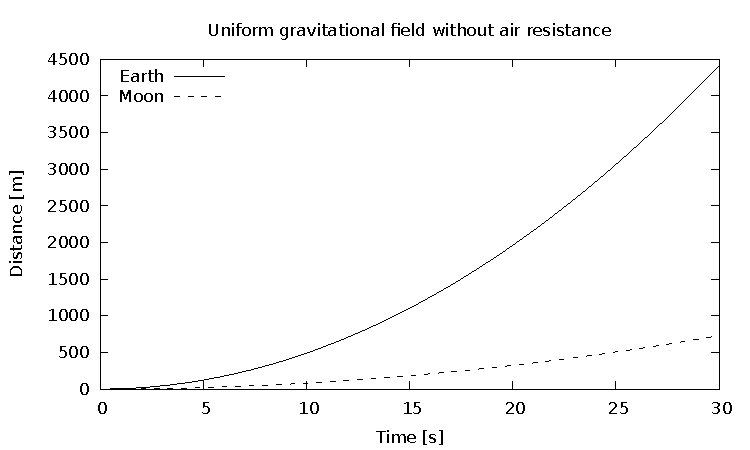
\includegraphics{gnuplot-bw}
 	\caption{Černobílá varianta obrázku generovaného programem Gnuplot}\label{fig:gnuplot-bw}
 \end{figure}
 
 \begin{figure}\centering
 	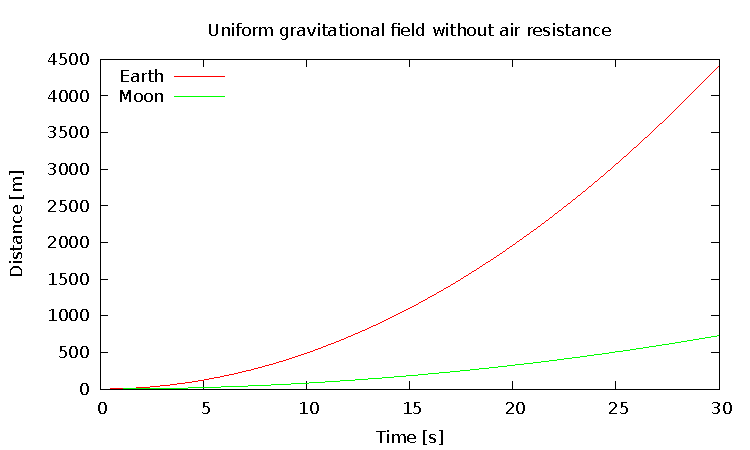
\includegraphics{gnuplot-col}
 	\caption{Barevná varianta obrázku generovaného programem Gnuplot}\label{fig:gnuplot-col}
 \end{figure}
 
 
 \subsection{Tabulky}
 
 Tabulky lze zadávat různě, např. v~prostředí \verb|tabular|, avšak pro jejich vkládání platí to samé, co pro obrázky -- použijte plovoucí prostředí, v~tomto případě \verb|table|. Například tabulka \ref{tab:matematika} byla vložena tímto způsobem.
 
 \begin{table}\centering
 	\caption[Příklad tabulky]{Zadávání matematiky}\label{tab:matematika}
 	\begin{tabular}{|l|l|c|c|}\hline
 		Typ		& Prostředí		& \LaTeX{}ovská zkratka	& \TeX{}ovská zkratka	\tabularnewline \hline \hline
 		Text		& \verb|math|		& \verb|\(...\)|	& \verb|$...$|		\tabularnewline \hline
 		Displayed	& \verb|displaymath|	& \verb|\[...\]|	& \verb|$$...$$|	\tabularnewline \hline
 	\end{tabular}
 \end{table}
 
% % % % % % % % % % % % % % % % % % % % % % % % % % % % 

\chapter{Obsah přiloženého CD}

\end{document}
